% Options for packages loaded elsewhere
\PassOptionsToPackage{unicode}{hyperref}
\PassOptionsToPackage{hyphens}{url}
%
\documentclass[
]{article}
\usepackage{amsmath,amssymb}
\usepackage{iftex}
\ifPDFTeX
  \usepackage[T1]{fontenc}
  \usepackage[utf8]{inputenc}
  \usepackage{textcomp} % provide euro and other symbols
\else % if luatex or xetex
  \usepackage{unicode-math} % this also loads fontspec
  \defaultfontfeatures{Scale=MatchLowercase}
  \defaultfontfeatures[\rmfamily]{Ligatures=TeX,Scale=1}
\fi
\usepackage{lmodern}
\ifPDFTeX\else
  % xetex/luatex font selection
\fi
% Use upquote if available, for straight quotes in verbatim environments
\IfFileExists{upquote.sty}{\usepackage{upquote}}{}
\IfFileExists{microtype.sty}{% use microtype if available
  \usepackage[]{microtype}
  \UseMicrotypeSet[protrusion]{basicmath} % disable protrusion for tt fonts
}{}
\makeatletter
\@ifundefined{KOMAClassName}{% if non-KOMA class
  \IfFileExists{parskip.sty}{%
    \usepackage{parskip}
  }{% else
    \setlength{\parindent}{0pt}
    \setlength{\parskip}{6pt plus 2pt minus 1pt}}
}{% if KOMA class
  \KOMAoptions{parskip=half}}
\makeatother
\usepackage{xcolor}
\usepackage[margin=1in]{geometry}
\usepackage{color}
\usepackage{fancyvrb}
\newcommand{\VerbBar}{|}
\newcommand{\VERB}{\Verb[commandchars=\\\{\}]}
\DefineVerbatimEnvironment{Highlighting}{Verbatim}{commandchars=\\\{\}}
% Add ',fontsize=\small' for more characters per line
\usepackage{framed}
\definecolor{shadecolor}{RGB}{248,248,248}
\newenvironment{Shaded}{\begin{snugshade}}{\end{snugshade}}
\newcommand{\AlertTok}[1]{\textcolor[rgb]{0.94,0.16,0.16}{#1}}
\newcommand{\AnnotationTok}[1]{\textcolor[rgb]{0.56,0.35,0.01}{\textbf{\textit{#1}}}}
\newcommand{\AttributeTok}[1]{\textcolor[rgb]{0.13,0.29,0.53}{#1}}
\newcommand{\BaseNTok}[1]{\textcolor[rgb]{0.00,0.00,0.81}{#1}}
\newcommand{\BuiltInTok}[1]{#1}
\newcommand{\CharTok}[1]{\textcolor[rgb]{0.31,0.60,0.02}{#1}}
\newcommand{\CommentTok}[1]{\textcolor[rgb]{0.56,0.35,0.01}{\textit{#1}}}
\newcommand{\CommentVarTok}[1]{\textcolor[rgb]{0.56,0.35,0.01}{\textbf{\textit{#1}}}}
\newcommand{\ConstantTok}[1]{\textcolor[rgb]{0.56,0.35,0.01}{#1}}
\newcommand{\ControlFlowTok}[1]{\textcolor[rgb]{0.13,0.29,0.53}{\textbf{#1}}}
\newcommand{\DataTypeTok}[1]{\textcolor[rgb]{0.13,0.29,0.53}{#1}}
\newcommand{\DecValTok}[1]{\textcolor[rgb]{0.00,0.00,0.81}{#1}}
\newcommand{\DocumentationTok}[1]{\textcolor[rgb]{0.56,0.35,0.01}{\textbf{\textit{#1}}}}
\newcommand{\ErrorTok}[1]{\textcolor[rgb]{0.64,0.00,0.00}{\textbf{#1}}}
\newcommand{\ExtensionTok}[1]{#1}
\newcommand{\FloatTok}[1]{\textcolor[rgb]{0.00,0.00,0.81}{#1}}
\newcommand{\FunctionTok}[1]{\textcolor[rgb]{0.13,0.29,0.53}{\textbf{#1}}}
\newcommand{\ImportTok}[1]{#1}
\newcommand{\InformationTok}[1]{\textcolor[rgb]{0.56,0.35,0.01}{\textbf{\textit{#1}}}}
\newcommand{\KeywordTok}[1]{\textcolor[rgb]{0.13,0.29,0.53}{\textbf{#1}}}
\newcommand{\NormalTok}[1]{#1}
\newcommand{\OperatorTok}[1]{\textcolor[rgb]{0.81,0.36,0.00}{\textbf{#1}}}
\newcommand{\OtherTok}[1]{\textcolor[rgb]{0.56,0.35,0.01}{#1}}
\newcommand{\PreprocessorTok}[1]{\textcolor[rgb]{0.56,0.35,0.01}{\textit{#1}}}
\newcommand{\RegionMarkerTok}[1]{#1}
\newcommand{\SpecialCharTok}[1]{\textcolor[rgb]{0.81,0.36,0.00}{\textbf{#1}}}
\newcommand{\SpecialStringTok}[1]{\textcolor[rgb]{0.31,0.60,0.02}{#1}}
\newcommand{\StringTok}[1]{\textcolor[rgb]{0.31,0.60,0.02}{#1}}
\newcommand{\VariableTok}[1]{\textcolor[rgb]{0.00,0.00,0.00}{#1}}
\newcommand{\VerbatimStringTok}[1]{\textcolor[rgb]{0.31,0.60,0.02}{#1}}
\newcommand{\WarningTok}[1]{\textcolor[rgb]{0.56,0.35,0.01}{\textbf{\textit{#1}}}}
\usepackage{graphicx}
\makeatletter
\def\maxwidth{\ifdim\Gin@nat@width>\linewidth\linewidth\else\Gin@nat@width\fi}
\def\maxheight{\ifdim\Gin@nat@height>\textheight\textheight\else\Gin@nat@height\fi}
\makeatother
% Scale images if necessary, so that they will not overflow the page
% margins by default, and it is still possible to overwrite the defaults
% using explicit options in \includegraphics[width, height, ...]{}
\setkeys{Gin}{width=\maxwidth,height=\maxheight,keepaspectratio}
% Set default figure placement to htbp
\makeatletter
\def\fps@figure{htbp}
\makeatother
\setlength{\emergencystretch}{3em} % prevent overfull lines
\providecommand{\tightlist}{%
  \setlength{\itemsep}{0pt}\setlength{\parskip}{0pt}}
\setcounter{secnumdepth}{-\maxdimen} % remove section numbering
\ifLuaTeX
  \usepackage{selnolig}  % disable illegal ligatures
\fi
\IfFileExists{bookmark.sty}{\usepackage{bookmark}}{\usepackage{hyperref}}
\IfFileExists{xurl.sty}{\usepackage{xurl}}{} % add URL line breaks if available
\urlstyle{same}
\hypersetup{
  pdftitle={HUDM6052 Psychometric II Homework\_02},
  pdfauthor={Chenguang Pan (cp3280@tc.columbia.edu)},
  hidelinks,
  pdfcreator={LaTeX via pandoc}}

\title{HUDM6052 Psychometric II Homework\_02}
\author{Chenguang Pan
(\href{mailto:cp3280@tc.columbia.edu}{\nolinkurl{cp3280@tc.columbia.edu}})}
\date{2023-09-28}

\begin{document}
\maketitle

\setcounter{tocdepth}{4}
\tableofcontents

\hypertarget{q1}{%
\subsection{Q1}\label{q1}}

\emph{Find the maximum discrimination for 1PL, 2PL, and 3PL logistic
models\ldots{}}

\textbf{My Solution:}\\
\textbf{2PL MODEL}

I begin with a 2PL model since 1PL is a special case of 2PL.

For the 2PL model, \[P(\theta)=\frac{1}{1+e^{-\alpha(\theta-\beta)}},\]
let \(Z = \alpha(\theta-\beta)\). Using the chain rule and take the
partial derivative on \(\alpha\), one can have
\[\frac{\partial P}{\partial \theta}=\frac{\partial P}{\partial Z}\frac{\partial Z}{\partial \theta}. \]
Then, expand the formula above, one can have
\[\frac{\partial P}{\partial \alpha}=P(1-P)\alpha.\] Note, this is the
slope function of a 2PL model, one still need to take the first
derivative (i.e., the second derivative of the original 2PL model) and
let it equal to 0 to get the local minimum or maximum. For
simplification, I use \(S(\theta)\) to represent the slope function of a
2PL model. Then, \[S(\theta) = \alpha P(1-P).\] Take the partial
derivative of the slope function, one can have
\[\frac{\partial S}{\partial\theta} = \frac{\partial S}{\partial P}\frac{\partial P}{\partial\theta} = (\alpha-2\alpha P)[\alpha P(1-P)]=0.\]
Solve the equation above, one can find that the extreme values of slope
occurs at \(P=0, P=1, P=\frac{1}{2}\). Rigorously, we still need to take
the second partial derivative of this slope function to determine the
whether it is the local minimum or maximum. But, from the ICC one can
easily find that slope will have maximum at \(P=\frac{1}{2}\). I skipped
this rigorous math proof here. Finally, solve the equation of
\(P(\theta)=\frac{1}{2}\), we can have the solution \(\theta = \beta\).

Therefore, the maximum value of discrimination of a 2PL model is at the
point \(\theta =\beta.\)

\textbf{1PL MODEL}

As for the 1PL model, plug the \(\alpha = 1\) into the partial
derivative of slope function \(\frac{\partial S}{\partial\theta}\)
above. One can easily have same conclusion that the maximum of slope of
1PL model is at the point \(\theta = \beta\).

\textbf{3PL MODEL}

\hypertarget{q2}{%
\subsection{Q2}\label{q2}}

\emph{Let the discrimination, difficulty and guessing parameters of five
items be\ldots{}}

\textbf{My Solution:}\\
First, I write a 3PL model function:

\begin{Shaded}
\begin{Highlighting}[]
\SpecialCharTok{\textgreater{}} \CommentTok{\# items\textquotesingle{} discrimination}
\ErrorTok{\textgreater{}}\NormalTok{ a\_ }\OtherTok{\textless{}{-}} \FunctionTok{c}\NormalTok{(}\FloatTok{0.5}\NormalTok{,}\DecValTok{1}\NormalTok{,}\FloatTok{1.5}\NormalTok{,}\FloatTok{2.5}\NormalTok{,}\DecValTok{1}\NormalTok{)}
\SpecialCharTok{\textgreater{}} \CommentTok{\# items\textquotesingle{} difficulty levels}
\ErrorTok{\textgreater{}}\NormalTok{ b\_ }\OtherTok{\textless{}{-}} \FunctionTok{c}\NormalTok{(}\SpecialCharTok{{-}}\DecValTok{1}\NormalTok{,}\SpecialCharTok{{-}}\FloatTok{0.5}\NormalTok{,}\DecValTok{0}\NormalTok{,}\FloatTok{0.5}\NormalTok{,}\DecValTok{1}\NormalTok{)}
\SpecialCharTok{\textgreater{}} \CommentTok{\# items\textquotesingle{}s guessing parameters}
\ErrorTok{\textgreater{}}\NormalTok{ c\_ }\OtherTok{\textless{}{-}} \FunctionTok{c}\NormalTok{(}\DecValTok{0}\NormalTok{,}\FloatTok{0.1}\NormalTok{,}\FloatTok{0.15}\NormalTok{,}\FloatTok{0.05}\NormalTok{,}\FloatTok{0.32}\NormalTok{)}
\SpecialCharTok{\textgreater{}} \CommentTok{\# trait vector}
\ErrorTok{\textgreater{}}\NormalTok{ theta\_ }\OtherTok{\textless{}{-}} \FunctionTok{c}\NormalTok{(}\SpecialCharTok{{-}}\FloatTok{2.0}\NormalTok{, }\SpecialCharTok{{-}}\FloatTok{1.0}\NormalTok{, }\DecValTok{0}\NormalTok{,}\DecValTok{1}\NormalTok{,}\DecValTok{2}\NormalTok{)}
\SpecialCharTok{\textgreater{}} \CommentTok{\# write a 3PL model}
\ErrorTok{\textgreater{}}\NormalTok{ irt\_3pl }\OtherTok{\textless{}{-}} \ControlFlowTok{function}\NormalTok{(theta,a,b,c)\{}
\SpecialCharTok{+}\NormalTok{   z }\OtherTok{\textless{}{-}} \FloatTok{1.702}\SpecialCharTok{*}\NormalTok{a}\SpecialCharTok{*}\NormalTok{(theta }\SpecialCharTok{{-}}\NormalTok{ b)}
\SpecialCharTok{+}\NormalTok{   output }\OtherTok{\textless{}{-}}\NormalTok{ c }\SpecialCharTok{+}\NormalTok{ (}\DecValTok{1}\SpecialCharTok{{-}}\NormalTok{c)}\SpecialCharTok{/}\NormalTok{(}\DecValTok{1}\SpecialCharTok{+}\FunctionTok{exp}\NormalTok{(}\SpecialCharTok{{-}}\NormalTok{z))}
\SpecialCharTok{+}   \FunctionTok{return}\NormalTok{(output)}
\SpecialCharTok{+}\NormalTok{ \}}
\end{Highlighting}
\end{Shaded}

Next, for each test-taker (i.e., each trait), get the required values
iteratively.

\begin{Shaded}
\begin{Highlighting}[]
\SpecialCharTok{\textgreater{}} \CommentTok{\# using a for{-}loop to get the values}
\ErrorTok{\textgreater{}} \ControlFlowTok{for}\NormalTok{ (j }\ControlFlowTok{in} \DecValTok{1}\SpecialCharTok{:}\DecValTok{5}\NormalTok{) \{}
\SpecialCharTok{+}   \CommentTok{\#print(paste0("{-}{-}{-}{-}{-}{-}{-}{-}{-}{-}{-}{-}{-}For the theta =", theta\_[j]," : {-}{-}{-}{-}{-}{-}{-}{-}{-}{-}{-}{-}{-}"))}
\SpecialCharTok{+}\NormalTok{   exp\_cor }\OtherTok{\textless{}{-}} \DecValTok{0}
\SpecialCharTok{+}   \ControlFlowTok{for}\NormalTok{ (i }\ControlFlowTok{in} \DecValTok{1}\SpecialCharTok{:}\DecValTok{5}\NormalTok{) \{}
\SpecialCharTok{+}     \CommentTok{\#print(paste0("{-}{-}{-}{-}{-}For the item i=", i," : {-}{-}{-}{-}{-}"))}
\SpecialCharTok{+}\NormalTok{     P }\OtherTok{\textless{}{-}} \FunctionTok{irt\_3pl}\NormalTok{(}\AttributeTok{theta=}\NormalTok{ theta\_[j], }
\SpecialCharTok{+}                  \AttributeTok{a=}\NormalTok{a\_[i], }\AttributeTok{b=}\NormalTok{b\_[i], }\AttributeTok{c=}\NormalTok{c\_[i])}
\SpecialCharTok{+}\NormalTok{     Q }\OtherTok{\textless{}{-}} \DecValTok{1}\SpecialCharTok{{-}}\NormalTok{P}
\SpecialCharTok{+}     \CommentTok{\# get the odds}
\SpecialCharTok{+}\NormalTok{     odds }\OtherTok{\textless{}{-}} \FunctionTok{round}\NormalTok{(P}\SpecialCharTok{/}\NormalTok{Q,}\DecValTok{3}\NormalTok{)}
\SpecialCharTok{+}     \CommentTok{\# get the logit}
\SpecialCharTok{+}\NormalTok{     logit }\OtherTok{\textless{}{-}} \FunctionTok{round}\NormalTok{(}\FunctionTok{log}\NormalTok{(odds),}\DecValTok{3}\NormalTok{)    }
\SpecialCharTok{+}     \CommentTok{\# if the odds greater than 1, we can expected this student j may}
\SpecialCharTok{+}     \CommentTok{\# get this item correctly}
\SpecialCharTok{+}     \ControlFlowTok{if}\NormalTok{(odds }\SpecialCharTok{\textgreater{}=}\DecValTok{1}\NormalTok{)\{}
\SpecialCharTok{+}\NormalTok{       exp\_cor }\OtherTok{\textless{}{-}}\NormalTok{ exp\_cor }\SpecialCharTok{+} \DecValTok{1}
\SpecialCharTok{+}\NormalTok{     \}}
\SpecialCharTok{+}     \CommentTok{\# print the results for this student}
\SpecialCharTok{+}     \CommentTok{\#print(paste0("Odds: ", odds," ."))}
\SpecialCharTok{+}     \CommentTok{\#print(paste0("Logit:", logit," ."))}
\SpecialCharTok{+}\NormalTok{   \}}
\SpecialCharTok{+}   \CommentTok{\# get the expected proportion of correct}
\SpecialCharTok{+}\NormalTok{   prop }\OtherTok{\textless{}{-}} \FunctionTok{round}\NormalTok{(exp\_cor}\SpecialCharTok{/}\DecValTok{5}\NormalTok{,}\DecValTok{3}\NormalTok{)}
\SpecialCharTok{+}   \CommentTok{\#print(paste0("Expected Correct \#:", exp\_cor," ."))}
\SpecialCharTok{+}   \CommentTok{\#print(paste0("Expected Correct proportion:", prop," ."))}
\SpecialCharTok{+}\NormalTok{ \}}
\end{Highlighting}
\end{Shaded}

To make the layout in a good-looking manner, I loaded the results from
above to a table as followed. Please remove the comment mark \texttt{\#}
before \texttt{print()} function to see the returned results.\\
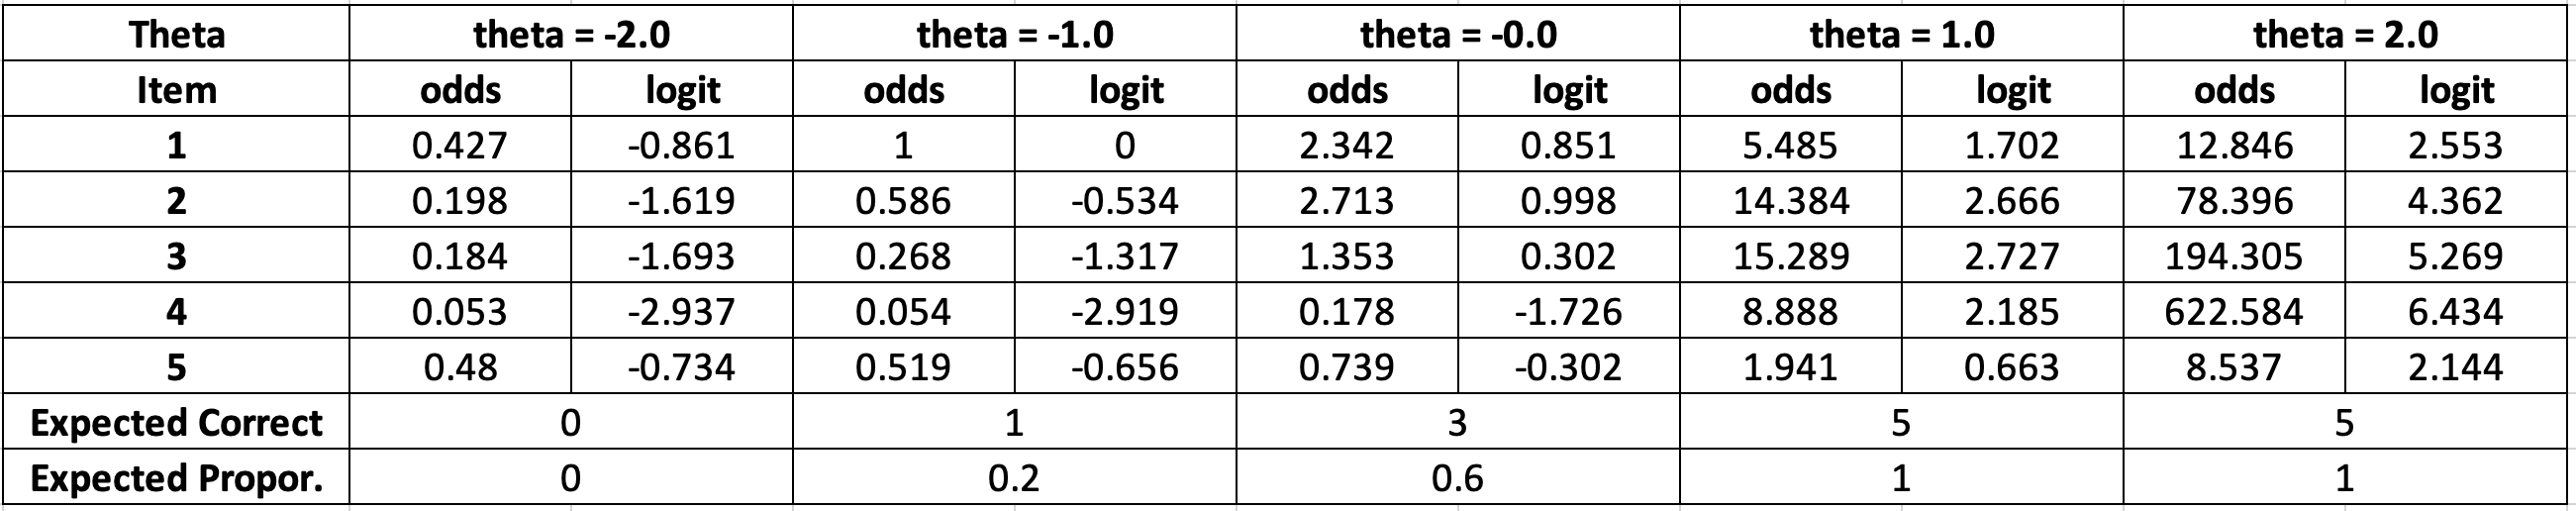
\includegraphics{table_1.png}

\hypertarget{q3-part-a}{%
\subsection{Q3-Part a}\label{q3-part-a}}

\emph{Find the maximum likelihood estimates of the item parameters
under\ldots{}}

\textbf{My Solution}

\begin{Shaded}
\begin{Highlighting}[]
\SpecialCharTok{\textgreater{}} \CommentTok{\# load the given values}
\ErrorTok{\textgreater{}} \DocumentationTok{\#\# the assumed theta\_j}
\ErrorTok{\textgreater{}}\NormalTok{ theta\_set }\OtherTok{\textless{}{-}} \FunctionTok{seq}\NormalTok{(}\SpecialCharTok{{-}}\DecValTok{3}\NormalTok{,}\DecValTok{3}\NormalTok{,}\AttributeTok{by =}\FloatTok{0.5}\NormalTok{)}
\SpecialCharTok{\textgreater{}} \DocumentationTok{\#\# number of correct responses for each theta\_j}
\ErrorTok{\textgreater{}}\NormalTok{ r\_set }\OtherTok{\textless{}{-}} \FunctionTok{c}\NormalTok{(}\DecValTok{0}\NormalTok{,}\DecValTok{0}\NormalTok{,}\DecValTok{1}\NormalTok{,}\DecValTok{2}\NormalTok{,}\DecValTok{3}\NormalTok{,}\DecValTok{4}\NormalTok{,}\DecValTok{5}\NormalTok{,}\DecValTok{6}\NormalTok{,}\DecValTok{4}\NormalTok{,}\DecValTok{4}\NormalTok{,}\DecValTok{4}\NormalTok{,}\DecValTok{2}\NormalTok{,}\DecValTok{1}\NormalTok{)}
\SpecialCharTok{\textgreater{}} \DocumentationTok{\#\# number of respondents for each theta\_j}
\ErrorTok{\textgreater{}}\NormalTok{ f\_set }\OtherTok{\textless{}{-}} \FunctionTok{c}\NormalTok{(}\DecValTok{1}\NormalTok{,}\DecValTok{2}\NormalTok{,}\DecValTok{4}\NormalTok{,}\DecValTok{7}\NormalTok{,}\DecValTok{8}\NormalTok{,}\DecValTok{9}\NormalTok{,}\DecValTok{10}\NormalTok{,}\DecValTok{8}\NormalTok{,}\DecValTok{6}\NormalTok{,}\DecValTok{5}\NormalTok{,}\DecValTok{5}\NormalTok{,}\DecValTok{2}\NormalTok{,}\DecValTok{1}\NormalTok{)}
\SpecialCharTok{\textgreater{}} 
\ErrorTok{\textgreater{}} \CommentTok{\# get the proportion of correct responses for each theta\_j}
\ErrorTok{\textgreater{}}\NormalTok{ p\_set }\OtherTok{\textless{}{-}}\NormalTok{ r\_set}\SpecialCharTok{/}\NormalTok{f\_set}
\SpecialCharTok{\textgreater{}} 
\ErrorTok{\textgreater{}} \CommentTok{\# to count the iteration times}
\ErrorTok{\textgreater{}}\NormalTok{ iter\_time }\OtherTok{\textless{}{-}} \DecValTok{0}
\SpecialCharTok{\textgreater{}}\NormalTok{ deltas }\OtherTok{\textless{}{-}} \FunctionTok{t}\NormalTok{(}\FunctionTok{t}\NormalTok{(}\FunctionTok{c}\NormalTok{(}\DecValTok{10}\NormalTok{,}\DecValTok{10}\NormalTok{)))}
\SpecialCharTok{\textgreater{}}\NormalTok{ zeta }\OtherTok{\textless{}{-}} \DecValTok{0}
\SpecialCharTok{\textgreater{}}\NormalTok{ lambda }\OtherTok{\textless{}{-}} \FloatTok{1.0}
\SpecialCharTok{\textgreater{}} 
\ErrorTok{\textgreater{}} \ControlFlowTok{while}\NormalTok{((}\FunctionTok{abs}\NormalTok{(deltas[}\DecValTok{1}\NormalTok{,}\DecValTok{1}\NormalTok{])}\SpecialCharTok{\textgreater{}}\FloatTok{0.005}\NormalTok{) }\SpecialCharTok{\&}\NormalTok{ (}\FunctionTok{abs}\NormalTok{(deltas[}\DecValTok{2}\NormalTok{,}\DecValTok{1}\NormalTok{])}\SpecialCharTok{\textgreater{}}\FloatTok{0.005}\NormalTok{)) \{}
\SpecialCharTok{+}   \CommentTok{\# set the initial value}
\SpecialCharTok{+}\NormalTok{   iter\_time }\OtherTok{\textless{}{-}}\NormalTok{ iter\_time}\SpecialCharTok{+}\DecValTok{1}
\SpecialCharTok{+}   \CommentTok{\# define the 2PL model:}
\SpecialCharTok{+}   \CommentTok{\# note, both the input and output are vectors rather than scalars}
\SpecialCharTok{+}\NormalTok{   P }\OtherTok{\textless{}{-}} \DecValTok{1}\SpecialCharTok{/}\NormalTok{(}\DecValTok{1}\SpecialCharTok{+}\FunctionTok{exp}\NormalTok{(}\SpecialCharTok{{-}}\NormalTok{(zeta}\SpecialCharTok{+}\NormalTok{lambda}\SpecialCharTok{*}\NormalTok{theta\_set)))}
\SpecialCharTok{+}\NormalTok{   Q }\OtherTok{\textless{}{-}} \DecValTok{1}\SpecialCharTok{{-}}\NormalTok{P}
\SpecialCharTok{+}   
\SpecialCharTok{+}   \CommentTok{\# define the weight in case of using normal ogive in the future}
\SpecialCharTok{+}\NormalTok{   W }\OtherTok{\textless{}{-}}\NormalTok{ P}\SpecialCharTok{*}\NormalTok{Q}
\SpecialCharTok{+}   
\SpecialCharTok{+}   \CommentTok{\# Define the L1, L11, L2, L22, L12}
\SpecialCharTok{+}   \CommentTok{\# Note, to make computation efficient, I use matrix operation}
\SpecialCharTok{+}\NormalTok{   vec\_tempt\_1 }\OtherTok{\textless{}{-}}\NormalTok{ (p\_set }\SpecialCharTok{{-}}\NormalTok{P)}\SpecialCharTok{/}\NormalTok{(P}\SpecialCharTok{*}\NormalTok{Q)}
\SpecialCharTok{+}\NormalTok{   vec\_tempt\_2 }\OtherTok{\textless{}{-}}\NormalTok{ (p\_set }\SpecialCharTok{{-}}\NormalTok{P)}\SpecialCharTok{*}\NormalTok{theta\_set}\SpecialCharTok{/}\NormalTok{(P}\SpecialCharTok{*}\NormalTok{Q)}
\SpecialCharTok{+}\NormalTok{   theta\_sq\_vec }\OtherTok{\textless{}{-}}\NormalTok{ theta\_set}\SpecialCharTok{\^{}}\DecValTok{2}
\SpecialCharTok{+}\NormalTok{   L1 }\OtherTok{\textless{}{-}} \FunctionTok{t}\NormalTok{(f\_set)}\SpecialCharTok{\%*\%}\FunctionTok{diag}\NormalTok{(W)}\SpecialCharTok{\%*\%}\FunctionTok{t}\NormalTok{(}\FunctionTok{t}\NormalTok{(vec\_tempt\_1))}
\SpecialCharTok{+}\NormalTok{   L2 }\OtherTok{\textless{}{-}} \FunctionTok{t}\NormalTok{(f\_set)}\SpecialCharTok{\%*\%}\FunctionTok{diag}\NormalTok{(W)}\SpecialCharTok{\%*\%}\FunctionTok{t}\NormalTok{(}\FunctionTok{t}\NormalTok{(vec\_tempt\_2))}
\SpecialCharTok{+}\NormalTok{   L11 }\OtherTok{\textless{}{-}} \SpecialCharTok{{-}}\FunctionTok{t}\NormalTok{(f\_set)}\SpecialCharTok{\%*\%}\FunctionTok{t}\NormalTok{(}\FunctionTok{t}\NormalTok{(W))}
\SpecialCharTok{+}\NormalTok{   L22 }\OtherTok{\textless{}{-}} \SpecialCharTok{{-}}\FunctionTok{t}\NormalTok{(f\_set)}\SpecialCharTok{\%*\%}\FunctionTok{diag}\NormalTok{(W)}\SpecialCharTok{\%*\%}\FunctionTok{t}\NormalTok{(}\FunctionTok{t}\NormalTok{(theta\_sq\_vec))}
\SpecialCharTok{+}\NormalTok{   L12 }\OtherTok{\textless{}{-}} \SpecialCharTok{{-}}\FunctionTok{t}\NormalTok{(f\_set)}\SpecialCharTok{\%*\%}\FunctionTok{diag}\NormalTok{(W)}\SpecialCharTok{\%*\%}\FunctionTok{t}\NormalTok{(}\FunctionTok{t}\NormalTok{(theta\_set))}
\SpecialCharTok{+}   
\SpecialCharTok{+}   \CommentTok{\# make them into matrix form}
\SpecialCharTok{+}\NormalTok{   matrix\_L }\OtherTok{\textless{}{-}} \FunctionTok{matrix}\NormalTok{(}\FunctionTok{c}\NormalTok{(L11,L12,L12,L22),}\DecValTok{2}\NormalTok{,}\DecValTok{2}\NormalTok{)}
\SpecialCharTok{+}\NormalTok{   vector\_L }\OtherTok{\textless{}{-}} \FunctionTok{t}\NormalTok{(}\FunctionTok{t}\NormalTok{(}\FunctionTok{c}\NormalTok{(L1, L2)))}
\SpecialCharTok{+}   
\SpecialCharTok{+}   \CommentTok{\# get the delta zeta and delta lambda}
\SpecialCharTok{+}\NormalTok{   deltas }\OtherTok{\textless{}{-}} \SpecialCharTok{{-}}\FunctionTok{solve}\NormalTok{(matrix\_L)}\SpecialCharTok{\%*\%}\NormalTok{vector\_L}
\SpecialCharTok{+}   
\SpecialCharTok{+}   \CommentTok{\# update the zeta and lambda}
\SpecialCharTok{+}   \CommentTok{\# note here is to add the deltas not to minus!!!!}
\SpecialCharTok{+}\NormalTok{   updated\_parameters }\OtherTok{\textless{}{-}} \FunctionTok{t}\NormalTok{(}\FunctionTok{t}\NormalTok{(}\FunctionTok{c}\NormalTok{(zeta, lambda))) }\SpecialCharTok{+}\NormalTok{ deltas}
\SpecialCharTok{+}\NormalTok{   zeta }\OtherTok{\textless{}{-}}\NormalTok{updated\_parameters[}\DecValTok{1}\NormalTok{,}\DecValTok{1}\NormalTok{]}
\SpecialCharTok{+}\NormalTok{   lambda }\OtherTok{\textless{}{-}}\NormalTok{ updated\_parameters[}\DecValTok{2}\NormalTok{,}\DecValTok{1}\NormalTok{]}
\SpecialCharTok{+}\NormalTok{ \}}
\SpecialCharTok{\textgreater{}} \FunctionTok{print}\NormalTok{(deltas[}\DecValTok{1}\NormalTok{])}
\NormalTok{[}\DecValTok{1}\NormalTok{] }\SpecialCharTok{{-}}\FloatTok{0.0001296827}
\SpecialCharTok{\textgreater{}} \FunctionTok{print}\NormalTok{(deltas[}\DecValTok{2}\NormalTok{])}
\NormalTok{[}\DecValTok{1}\NormalTok{] }\FloatTok{0.000476612}
\SpecialCharTok{\textgreater{}} \FunctionTok{print}\NormalTok{(}\FunctionTok{paste0}\NormalTok{(}\StringTok{"The iteration time is: "}\NormalTok{, iter\_time,}\StringTok{" ."}\NormalTok{))}
\NormalTok{[}\DecValTok{1}\NormalTok{] }\StringTok{"The iteration time is: 3 ."}
\SpecialCharTok{\textgreater{}} \FunctionTok{print}\NormalTok{(}\FunctionTok{paste0}\NormalTok{(}\StringTok{"The estimated zeta is: "}\NormalTok{, }\FunctionTok{round}\NormalTok{(zeta,}\DecValTok{4}\NormalTok{),}\StringTok{" ."}\NormalTok{))}
\NormalTok{[}\DecValTok{1}\NormalTok{] }\StringTok{"The estimated zeta is: 0.2016 ."}
\SpecialCharTok{\textgreater{}} \FunctionTok{print}\NormalTok{(}\FunctionTok{paste0}\NormalTok{(}\StringTok{"The estimated lambda is: "}\NormalTok{, }\FunctionTok{round}\NormalTok{(lambda,}\DecValTok{4}\NormalTok{),}\StringTok{" ."}\NormalTok{))}
\NormalTok{[}\DecValTok{1}\NormalTok{] }\StringTok{"The estimated lambda is: 0.8236 ."}
\end{Highlighting}
\end{Shaded}

The results show that the \(\hat{\zeta}=.202\) and
\(\hat{\lambda}=.824\) after 4 iterations. Convert the value into
\(\hat{\alpha} = \hat{\lambda}=.824\) and
\(\hat{\beta} = -\frac{\hat{\zeta}}{\hat{\lambda}}=-0.245\). Therefore,
the estimated logistic model is
\[P(\theta)=\frac{1}{1+e^{-.824(\theta+.245)}}.\]

Notes about coding: The way my code to get the \texttt{L1},\texttt{L11},
etc., is kinda wordy. R actually provides more efficient way. For
example, one can just type
\texttt{L1\ \textless{}-\ sum(f\_set*W*vec\_tempt\_1)} to get the same
result. Here, I use the matrix alegra style to refresh my memory about
the past math knowledge.

\end{document}
